\parskip=1cm
\parindent=0pt

A small image with a filled circle follows here (with baseline): \tikz[baseline] \fill[red] (0,1cm) circle(2pt);

\tikzsetnextfilename{\tikzexternalrealjob-setnextfilename}
The next one uses 

\begin{tikzpicture}[baseline]
	\draw (0,0) grid (4,4);
\end{tikzpicture}
an explizit file name.

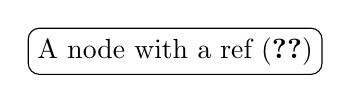
\begin{tikzpicture}
	\node[draw,rounded corners] {A node with a ref (\ref{eq:1})};
\end{tikzpicture}

\begin{equation}
	1+1=3
	\label{eq:1}
\end{equation}


\begin{tikzpicture}
	\node[draw,rounded corners] {A node which contains a label\label{a:label:in:a:picture}};
\end{tikzpicture}

The label inside of a node is on page~\pageref{a:label:in:a:picture}.

\expandafter\ifx\csname pgfplotslegendfromname\endcsname\relax
\else
The following picture exports a legend to the aux file (if possible).
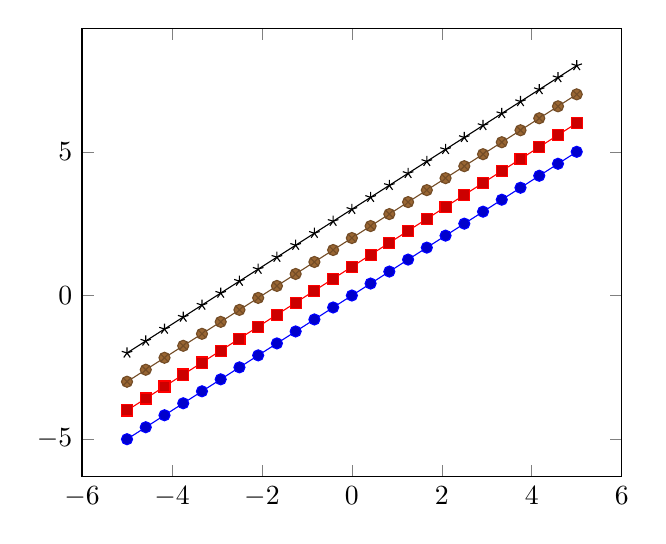
\begin{tikzpicture}
	\begin{axis}[legend entries={1,2,3,4},legend to name=legend:name]
	\addplot {x};
	\addplot {x+1};
	\addplot {x+2};
	\addplot {x+3};
	\end{axis}
\end{tikzpicture}

Here is the legend: \pgfplotslegendfromname{legend:name}.
\fi
